%%%%%%%%%%%%%%%%%%%%%%% file template.tex %%%%%%%%%%%%%%%%%%%%%%%%%
%
% This is a general template file for the LaTeX package SVJour3
% for Springer journals.          Springer Heidelberg 2010/09/16
%
% Copy it to a new file with a new name and use it as the basis
% for your article. Delete % signs as needed.
%
% This template includes a few options for different layouts and
% content for various journals. Please consult a previous issue of
% your journal as needed.
%
%%%%%%%%%%%%%%%%%%%%%%%%%%%%%%%%%%%%%%%%%%%%%%%%%%%%%%%%%%%%%%%%%%%
%
% First comes an example EPS file -- just ignore it and
% proceed on the \documentclass line
% your LaTeX will extract the file if required
%% \begin{filecontents*}{example.eps}
%% %!PS-Adobe-3.0 EPSF-3.0
%% %%BoundingBox: 19 19 221 221
%% %%CreationDate: Mon Sep 29 1997
%% %%Creator: programmed by hand (JK)
%% %%EndComments
%% gsave
%% newpath
%%   20 20 moveto
%%   20 220 lineto
%%   220 220 lineto
%%   220 20 lineto
%% closepath
%% 2 setlinewidth
%% gsave
%%   .4 setgray fill
%% grestore
%% stroke
%% grestore
%% \end{filecontents*}
%
\RequirePackage{fix-cm}
%
%\documentclass{svjour3}                     % onecolumn (standard format)
%\documentclass[smallcondensed]{svjour3}     % onecolumn (ditto)
\documentclass[smallextended]{svjour3}       % onecolumn (second format)
%\documentclass[twocolumn]{svjour3}          % twocolumn
%
\smartqed  % flush right qed marks, e.g. at end of proof
%
\usepackage{graphicx}
%
% \usepackage{mathptmx}      % use Times fonts if available on your TeX system
%
% insert here the call for the packages your document requires
%\usepackage{latexsym}
% etc.
%
% please place your own definitions here and don't use \def but
% \newcommand{}{}
%
% Insert the name of "your journal" with
\journalname{Cyber Security T\&L-2018}
%
\begin{document}

\title{A laboratory environment with honeypots for teaching cyber-security in H.E.%\thanks{Grants or other notes
%about the article that should go on the front page should be
%placed here. General acknowledgments should be placed at the end of the article.}
}
%\subtitle{Do you have a subtitle?\\ If so, write it here}

\titlerunning{Honeypots in H.E. teaching}        % if too long for running head

\author{Dr~Neil~Eliot \and
        Dr~David~Kendall \and
        Dr~Michael~Brockway
}

%\authorrunning{Short form of author list} % if too long for running head

\institute{Dr N. Eliot \at
              Northumbria University \\
              \email{neil.eliot@northumbria.ac.uk}           %  \\
           \and
           Dr D. Kendall \at
              Northumbria University \\
              \email{david.kendall@northumbria.ac.uk}           %  \\
           \and
           Dr M. Brockway \at
              Northumbria University \\
              \email{david.kendall@northumbria.ac.uk}           %  \\
}

\date{Received: date / Accepted: date}
% The correct dates will be entered by the editor


\maketitle

\begin{abstract}
Teaching cyber-security within a University environment requires a closed environment that is off-campus and configured such that students can transfer theoretical principles into practical cyber-security skills. The subject necessitates the need for honeypot technologies that will allow the investigation of network-based cyber-security attacks. The need for a closed environment, which may be considered as a ``sandbox'', arises from the nature of cyber-security investigations, especially where students are required to investigate network protocol-based attacks that could render a teaching network environment unstable or unusable. 

Although the environments are closed they still require access to the internet. The honeypot platform and the teaching environments discussed in this paper are designed so as to provide an environment that is flexible enough to allow the teaching of general purpose networking and operating systems subjects, and to support complex sand-boxed integration of honeypot technologies for the teaching of the practical aspects of cyber-security. 

The paper concludes by outlining how the platform has been successfully deployed within a University environment to support undergraduate and postgraduate teaching and learning by highlighting the types of experimentation and projects that the environment has supported and will support in the future.
\keywords{Cyber Security \and Network Security \and Honeypot}
% \PACS{PACS code1 \and PACS code2 \and more}
% \subclass{MSC code1 \and MSC code2 \and more}
\end{abstract}

\section{Introduction}\label{intro}
When teaching cyber-security in an academic environment there are many considerations that need to be taken into account, not least, respecting other users privacy and their access to the learning and teaching facilities within the academic environment.

Activities such as reconnaissance and experimentation can result in traffic or services being deployed into the teaching network environment. These activities may effect other users through service depletion, traffic redirection~\cite{ACGO:06,LR:06} or through data capture that may compromise a users legal rights e.g. capturing activity or sensitive information that you are not authorised to possess.

The environment must also support activities that would normally be prevented through configurations designed for production environments. A \emph{normal} academic infrastructure designed for general student access may implement restrictions through \texttt{MAC} blocking to prevent rogue equipment being attached to the network or firewalls to prevent access to to specific internet sites. From a cyber-security teaching perspective this would severely limit the scope of the technologies that could be deployed and investigated and limit access to potential teaching resources~\cite{ACGO:06,YYLCHJ:04}. Also a general purpose network deployment would not provide students with the administrative privileges that are required.

When investigating cyber-security there is also a need for the environment to be controlled such that the services and network protocols are minimised or reduced  therefore the effects an attack have upon the environment can be isolated and analyses effectively i.e. if analysing the effects of throughput on a protocol any rogue activities, such as file transfers or service advertising may impact on the experimental environment and invalidate the results.

These issues highlight the need for a clear definition of the requirements of \emph{academic honeypot} environments and the need for closed specialist environments for the study of cyber-security.

Honeypots are computer systems that are specifically designed for cyber-security investigations~\cite{FKAS:17,BCF:12,ZZQL:03}. They can be full network deployments incorporating switches, routers, and multiple servers providing network services or they can be a program running on a single machine. Honeypots fall into two distinct categories: 

\begin{itemize}
\item \noindent \emph{\textbf{Low Interaction:}} This type of honeypot implements a course grain service capturing a low level of detail, it can also be used to act as a distractor for a bot-based attack~\cite{SZB:16}.
\newline
\item \noindent \emph{\textbf{High Interaction:}} This type of honeypot allows fine grained data capture and in-depth analysis of a system as it reacts to usage. This type of honeypot is also cited as a ``research'' honeypot as discussed by Mairh et al.~\cite{MBVJ:11}. High-interaction honeypots can also be used to distract potential hackers from a genuine system (a decoy)~\cite{M:06,SNKA:12}. 
\end{itemize}

Honeypots can be deployed into different load-based environments depending upon the type of analysis work that is being investigated. The loading activity can be categorised in two ways:
 
\begin{itemize}
\item \noindent \emph{\textbf{Low Volume}} A honeypot deployed in a research laboratory to investigate the effect of a small number of concurrent requests is a low volume honeypot.
\item \noindent \emph{\textbf{High Volume}} A honeypot capable of being deployed in an environment that results in the honeypot being subjected to high levels of usage specifically to analyse the effects of a large number of concurrent requests from multiple sources is a high volume honeypot.
\end{itemize}
 
These two categories provide four different types of honeypot based upon interaction and loading (Volume). These categories are shown in Table~\ref{table:HoneypotTypes}.

\begin{table}[h]
\begin{center}
\begin{tabular}{ | c | c| c | } 
\hline
 & High Volume & Low Volume\\ 
\hline
Low Interaction & \texttt{LIHV} & \texttt{LILV} \\ 
\hline
High Interaction & \texttt{HIHV} & \texttt{HILV} \\ 
\hline
\end{tabular}
\end{center}
\caption{Honeypot Type/Volume categorisation}
\label{table:HoneypotTypes}
\end{table}

This paper focuses on the use of \emph{H}igh-\emph{I}nteraction-\emph{L}ow-\emph{V}olume (\texttt{HILV}) and \emph{L}ow-\emph{I}nteraction-\emph{H}igh-\emph{V}olume (\texttt{LIHV}) honeypots and the requirements of an academic networking platform to support the delivery of both undergraduate and postgraduate cyber-security programmes. 

The two other types of honeypots are not required for undergraduate purposes, specifically \emph{H}igh-\emph{I}nteraction-\emph{H}igh-\emph{V}olume (\texttt{HIHV}) due to the cost of deployment and the length of time the environment would take to reconfigure for teaching purposes. This type of honeypot would be useful in a research environment such as a research centre for use in long term internet-based projects. The \emph{L}ow-\emph{I}nteraction-\emph{L}ow-\emph{V}olume (\texttt{LILV}) platform can be deployed inside the \texttt{HILV} platform as an academic exercise, for example installing and testing Kippo~\cite{D:16,SH:15}.

Romney and Lanoy~\cite{LR:06} discuss the use of virtual environments as a mechanism to deploy honeypot platforms, virtualisation as a technology can introduce limitations with respect to deployment, resource utilisation, and data capture. Aspects of the deployment discussed in this paper are similar to those of Romney and Lanoy but the focus in this paper is the use of honeypots for undergraduate and post-graduate students. The paper extends their work by deploying honeypot environments as a physical configuration to increase the potential use of the honeypots as a learning environment. Spitner~\cite{LS:03} discusses many cyber-security based attack techniques and the physically deployed \texttt{HILV} lends itself to the types of attacks he discusses. This includes deploying a \texttt{HILV} honeypot within the laboratory and allowing access from the laboratory to specific services or equipment within it to emulate ``real'' attacks. 

The honeypot designs in this paper extend the ability to deploy multi honeypot experimental environments as discussed by Duffany~\cite{JD:08}. This is achieved by reducing the cost of the honeypot architecture to increase the number of available honeypots for a distributed data capture deployment. The proposals in this paper also make the \texttt{LIHV} honeypot architecture small enough to be a portable device suitable for deployment in multiple locations.

\section{Teaching Requirements}\label{sec:TeachingRequire}

\subsection{General networking laboratory}\label{subsec:GeneralLab}
\noindent \emph{\textbf{Requirement 1:}} There must be a flexible re-configurable base laboratory environment, isolated from the main university campus network, for students to carry out their normal studies of networks, operating systems and network services. Students require administrative access to the basic networking equipment such as routers, switches, and desktop machines for installation and configuration of general purpose tools and virtual environments. These activities would normally be prohibited on a University campus network.
\newline\newline
\noindent \emph{\textbf{Requirement 2:}} The network needs to provide unfiltered access to the internet to allow access to security sites and software packages. Many academic networks block access to cyber-security tool sites from their specialist and general access laboratories~\cite{ACGO:06,YYLCHJ:04} as well as the open access areas used by students. Tools such a \texttt{Metasploit}~\cite{R7:17} or the \texttt{Kali Linux} distribution~\cite{OS:17} are usually blocked, as are cyber-security information sites such as \texttt{http://www.hak5.org} or \texttt{https://www.exploit-db.com/}.

\subsection{\texttt{LIHV} honeypot}\label{subsec:LabHoneypot}
\noindent \emph{\textbf{Requirement 3:}} There needs to be a facility that allows large numbers of students to test existing cyber-security tools and to provide them with the ability to develop and test their own tools. 

\subsection{\texttt{HILV} honeypot}\label{subsec:ResearchHoneypot}
\noindent \emph{\textbf{Requirement 4:}} There needs to be a mechanism that allows students to build environments that are connected to the general networking laboratory via port mapping or address forwarding. 
\newline\newline
\noindent \emph{\textbf{Requirement 5:}} The \texttt{HILV} honeypot must support deployment of basic networking services on multiple low-cost servers (\texttt{DHCP}/\texttt{DNS}/\texttt{HTTP}/\texttt{DB}) to allow inter-service communications to be analysed. 
\newline\newline
\noindent \emph{\textbf{Requirement 6:}} The servers need to be small scale low-cost machines with limited hardware resources to allow the analysis of resource exhaustion attacks where there are limited attacking end points e.g. a botnet consisting of a few machines rather than hundreds or thousands. 
\newline\newline
\noindent \emph{\textbf{Requirement 7:}} The honeypot must provide scope for additional services and devices to be added. It must also provide the ability to cascade multiple honeypots to create a honeynet~\cite{AA:15,FDF:15,KNC:15}.
\newline\newline
\noindent \emph{\textbf{Requirement 8:}} The honeypot must facilitate effective network traffic capture to ensure the integrity of any network analysis e.g. identifying network transactions in a website defacement or denial of service-based (\texttt{DoS} or \texttt{DDoS}) attack, or spoofed packets such as in \texttt{ARP} poisoning for man-in-the-middle (\texttt{MitM}) attacks~\cite{PS:16,RSKA:16}.  

\section{Logical/Physical network infrastructure}\label{LogicalDesign}

The teaching environment consists of three distinct components: The general networking laboratory (\textit{requirement 1,2}), the \texttt{LIHV} honeypot (\textit{requirement 3}) and the small scale \texttt{HILV} honeypots (\textit{requirements 4,5,6,7,8}). 

\subsection{General networking laboratory}
The flexible laboratory environment needs to provide a re-configurable physical networking layer. This is provided by a structured cabling architecture as shown in~Figure~\ref{fig:Overview1}. 

\begin{figure}[h]
\begin{center}
	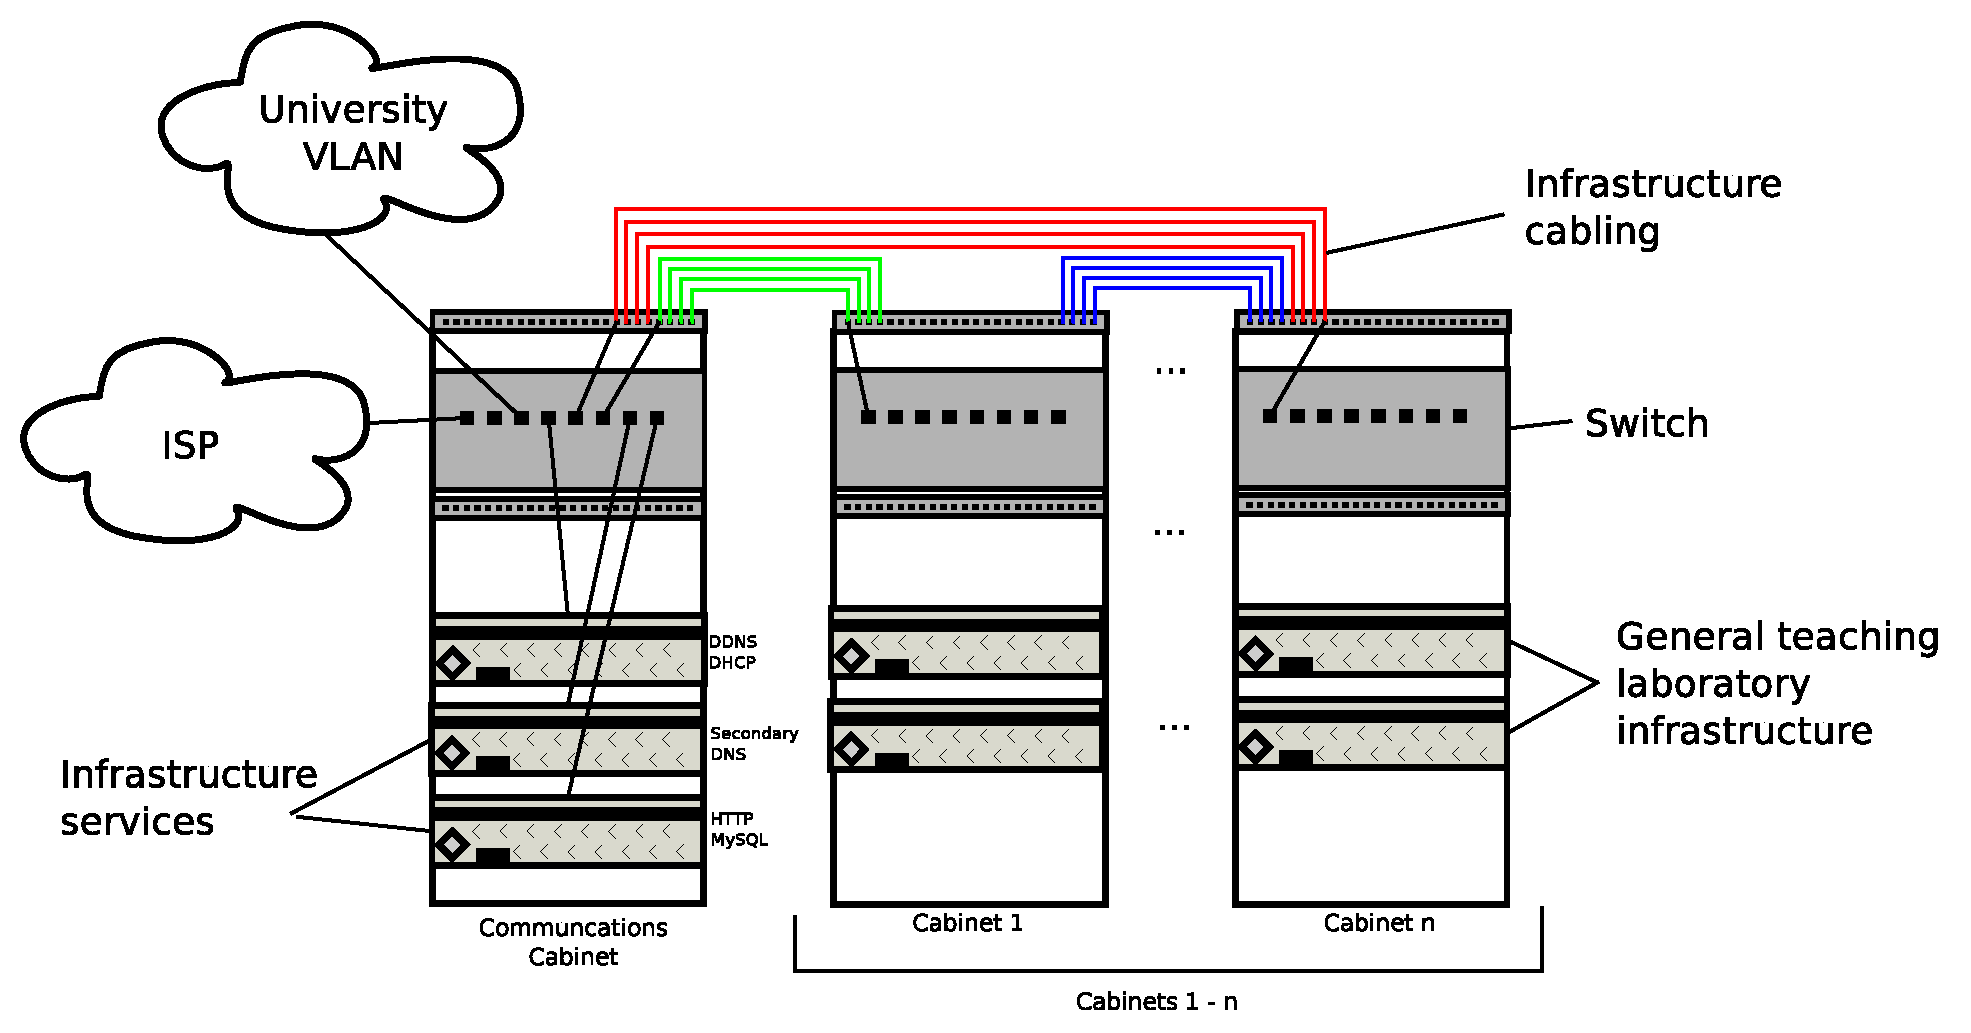
\includegraphics[scale=0.4]{Images/Infrastructure.eps}
\caption{General networking laboratory overview}
\label{fig:Overview1}
\end{center}
\end{figure}

The ``Communications Cabinet'' is secured; students are not allowed access, to prevent reconfiguration of the base network and the network services equipment. The cabinet contains the \texttt{DHCP} and \texttt{DNS} servers, a 1U intranet server, a database server and a \texttt{NAS} drive. The communication cabinet includes a \texttt{VDSL} fibre link from the \texttt{ISP}. In the case of Northumbria University the provider is BT Business~\cite{BT:17}. The router used to manage the \texttt{ISP} connection is a Draytek Vigor 2850~\cite{DC:17}.

Each of the cabinets are linked to a laboratory bench supporting 8 - 10 students. Each cabinet contains a selection of switches, routers, \texttt{IP} Telephony, \texttt{IDS}, and Firewall equipment that are required for general network architecture modules. These cabinets are linked back to the communications cabinet to provide internet access for the benches. Access to the internet from the desktop is achieved through a \texttt{NAT} connection from the communications cabinet \texttt{ISP} router. 

The structured cabling allows the resources of each cabinet within the laboratory to be linked to the desktop through four structured cabling ports. Cross-cabinet connections ensure specialist resources are flexibly available to all benches e.g. switches, routers, firewalls, and \texttt{IDS} (Intrusion Detection Systems) etc.

\subsection{Address range support}
The use of virtualisation (\texttt{GNS3}~\cite{GNS3:17}, VMWare~\cite{VMWARE:17} and VirtualBox~\cite{O:17}) to support the operating systems and networking modules necessitates a large number of host addresses, to support a large number of students deploying statically addressed virtual hosts. Running the base infrastructure as a single subnet allows freedom of movement of the laboratory equipment. Using a class B address provides 65,534 addresses which is enough for each student to be allocated a block of contiguous \texttt{IP} addresses for each module allowing multiple modules to be delivered concurrently without having \texttt{IP} address conflicts. 

\subsection{Network service deployment}\label{InfraService}
To support the operating systems and general computing subjects the network requires, as a minimum, \texttt{DNS}~\cite{RA:11} and \texttt{DHCP}~\cite{DL:02} services. These services two services are deployed across three small scale 1U servers (HPE ProLiant DL360 Gen9 Server~\cite{HPE:17}). Two servers are located in the communications cabinet as shown in~Figure~\ref{fig:Overview1}. One server supports \texttt{DHCP} and \texttt{DNS} which are integrated to create a \texttt{DDNS}~\cite{SV:06} environment. The second server acts as the secondary \texttt{DNS} server. The third server is located in the \texttt{LIHV} honeypot cabinet and acts as a further secondary \texttt{DNS} server. 

The communication cabinet also contains a 1U server that provides the laboratory intranet (\texttt{LAMP} based) service, along with a general purpose \texttt{MySQL} database services for the intranet and module content delivery. 

Deployment of known desktop equipment is coordinated by creating reservation entries in the \texttt{DHCP} service. The \texttt{DHCP} server then automatically creates the forward and reverse \texttt{DNS} entries in the \texttt{DNS} architecture as the equipment boots. Students can also connect their own devices which are allocated a network configuration from a \texttt{DHCP} address pool. 

\subsection{Teaching facilities support}
The teaching of the standard technologies such as switching and routing utilise the physical equipment within the cabinets. The laboratory also supports network virtualisation through \texttt{GNS3} which can be integrated with the physical equipment when necessary. The teaching of the \texttt{OS} based technologies is supported through the use of desktop virtualisation allowing each student to have multiple client and server technologies running simultaneously on a single machine. For large scale deployments, which is required on some modules, the deployment of the virtual machines is across several desktop machines. The large scale deployments require the virtualisation software to support network card bridging to allow the virtual machines to be ``physically" connected to the laboratory infrastructure. Subjects that require a laboratory ``search-by-name" facility (\texttt{DNS} and \texttt{rDNS}) such as Java Sockets and C Sockets programming are supported by the \texttt{DDNS} implementation as discussed in~Section~\ref{InfraService}.

\section{Honeypot architectures}

As shown in Table~\ref{table:HoneypotTypes} the four types are:
\begin{itemize}
\item \noindent \emph{\textbf{LIHV}} This type of honeypot is used when carrying out analysis of high levels of system interaction but only capturing a limited amount of service and system activity data for example analysing multiple attackers carrying out authentication attacks on an \texttt{FTP} server and only analysing the service log files. This type of honeypot can also be used in a general purpose networking laboratory with students to allow them to investigate authentication tools such as Hydra and xHydra~\cite{RS:15} and to be a target when they are developing their own tools such as an authentication based botnet. 

\item \noindent \emph{\textbf{LILV}} This type of honeypot is used when a basic testing platform is required to identify how a service is being attacked. There is no other interactions under investigation, for example using software systems such as Kippo~\cite{D:16,SH:15}, and testing how it logs transactions to a file or a database. There are a few login transactions from a limited number (usually 1) user and a simple activity log of attempted logins.

\item \noindent \emph{\textbf{HIHV}} This type of honeypot is used when a system is being thoroughly tested with high levels of user interaction (pressure testing) and involves large numbers of high power servers capable of supporting high levels of concurrent interactions. These honeypots provide detailed data capture capabilities of all the services and the inter-service interactions as well as system transactions e.g. \texttt{SQL} Queries and responses. They are usually deployed as a ``real'' system that is being penetration tested and they are often exposed to the internet to analyses the effects of unsolicited attacks.  

\item \noindent \emph{\textbf{HILV}} This type of honeypot is used when there is a low level of interaction with the system but the data captured is fine grain. For example investigating an enumeration attack such as a \texttt{DNS} query. The detail of the information gathered from the enumeration is low activity i.e. a single \texttt{AXFR}~\cite{EL:10} query., However the effect of the query and the activity it generates within the system is collected in great details. Another example would be profiling a \texttt{Wordpress}~\cite{WP:17} site using \texttt{WPScan}~\cite{WT:17}.

\end{itemize}

The two types of honeypot deployed into the laboratory are \emph{H}igh-\emph{I}nteraction-\emph{L}ow-\emph{V}olume (\texttt{HILV}) and the \emph{L}ow-\emph{I}nteraction-\emph{H}igh-\emph{V}olume (\texttt{LIHV}).

\subsection{\texttt{HILV} Honeypot}
The \texttt{HILV} honeypot architecture is an isolated environment. This is achieved by using a commercially available cable router that is connected to the main laboratory infrastructure as shown in Figure~\ref{fig:HPOverview}. 

\begin{figure}[!ht]
\begin{center}
	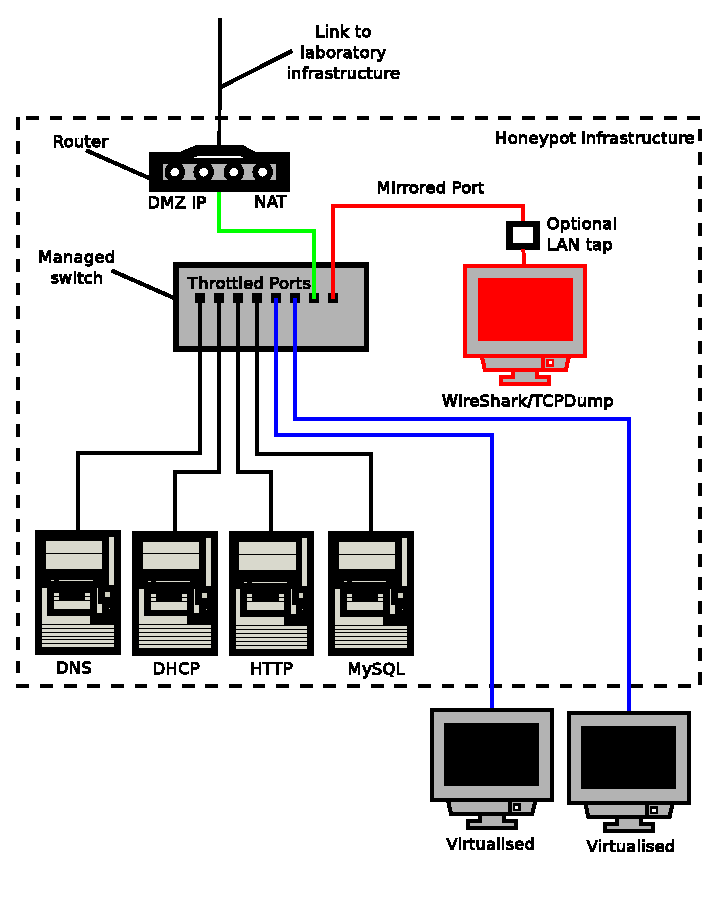
\includegraphics[scale=0.70]{Images/Honeypot1.eps}
\caption{\texttt{HILV} Honeypot overview}
\label{fig:HPOverview}
\end{center}
\end{figure}

Figures~\ref{fig:HP1}~and~\ref{fig:HP2} shows the complete device as deployed in the specialist teaching laboratories. The complete research honeypot consists of:

\begin{itemize}
\item \noindent A router for traffic management to and from the laboratory infrastructure via \texttt{NAT} and Address forwarding. (connected via the green cable).
\item \noindent 4 Raspberry Pi boards for service deployment.
\item \noindent A managed switch for packet capture:
\begin{itemize}
	\item \noindent 1 port (port 8) setup as a monitor usually connected to a PC running TCPDump or Wireshark (Red Cable).
	\item \noindent All other ports are mirrored to the monitor (ports 1-7). 
	\item \noindent 1 port (port 1) cascades to the router. 
	\item \noindent 4 ports are connected to the 4 Raspberry Pi servers (ports 2-5) cascades to the router. 
	\item \noindent 2 spare ports (ports 6,7) are available for additional services or clients to be added (Blue Cables)
\end{itemize}
\end{itemize}

\begin{figure}[ht]
  \centering
  \begin{minipage}[h]{0.45\textwidth}
    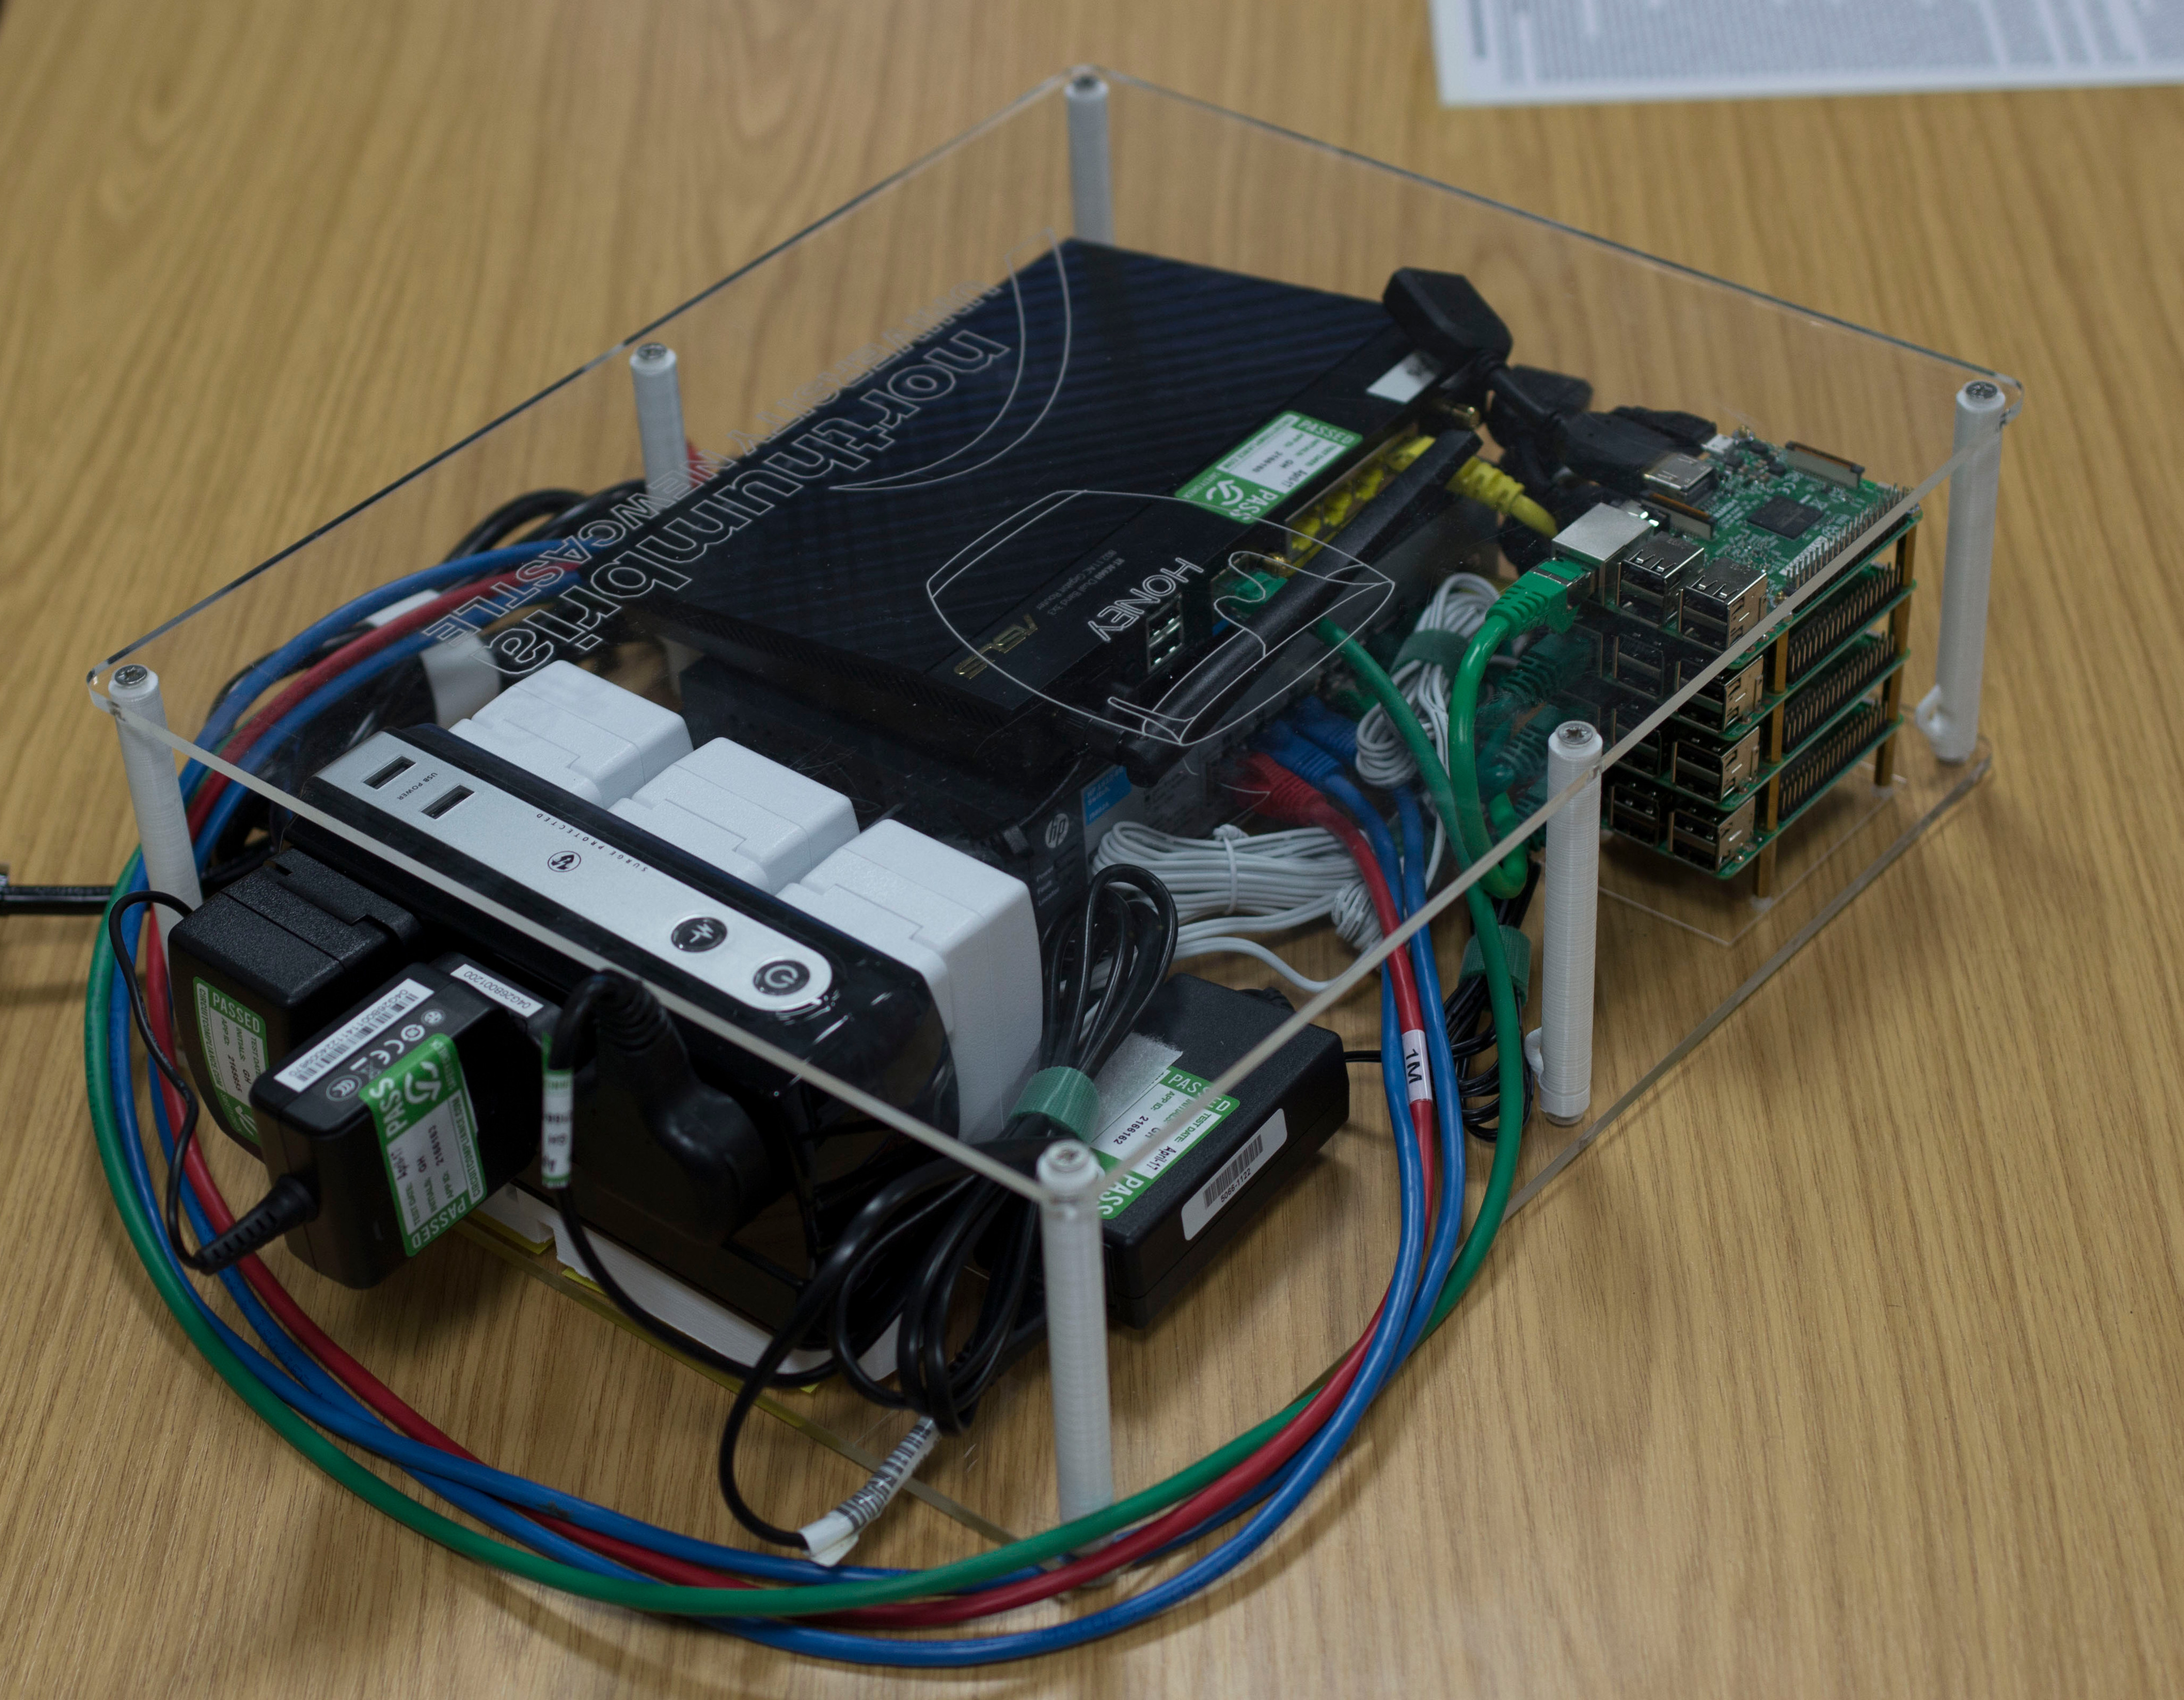
\includegraphics[width=\textwidth]{Images/HP1.eps}
    \caption{\texttt{HILV} side view}
    \label{fig:HP1}
  \end{minipage}
  \hfill
  \begin{minipage}[h]{0.45\textwidth}
    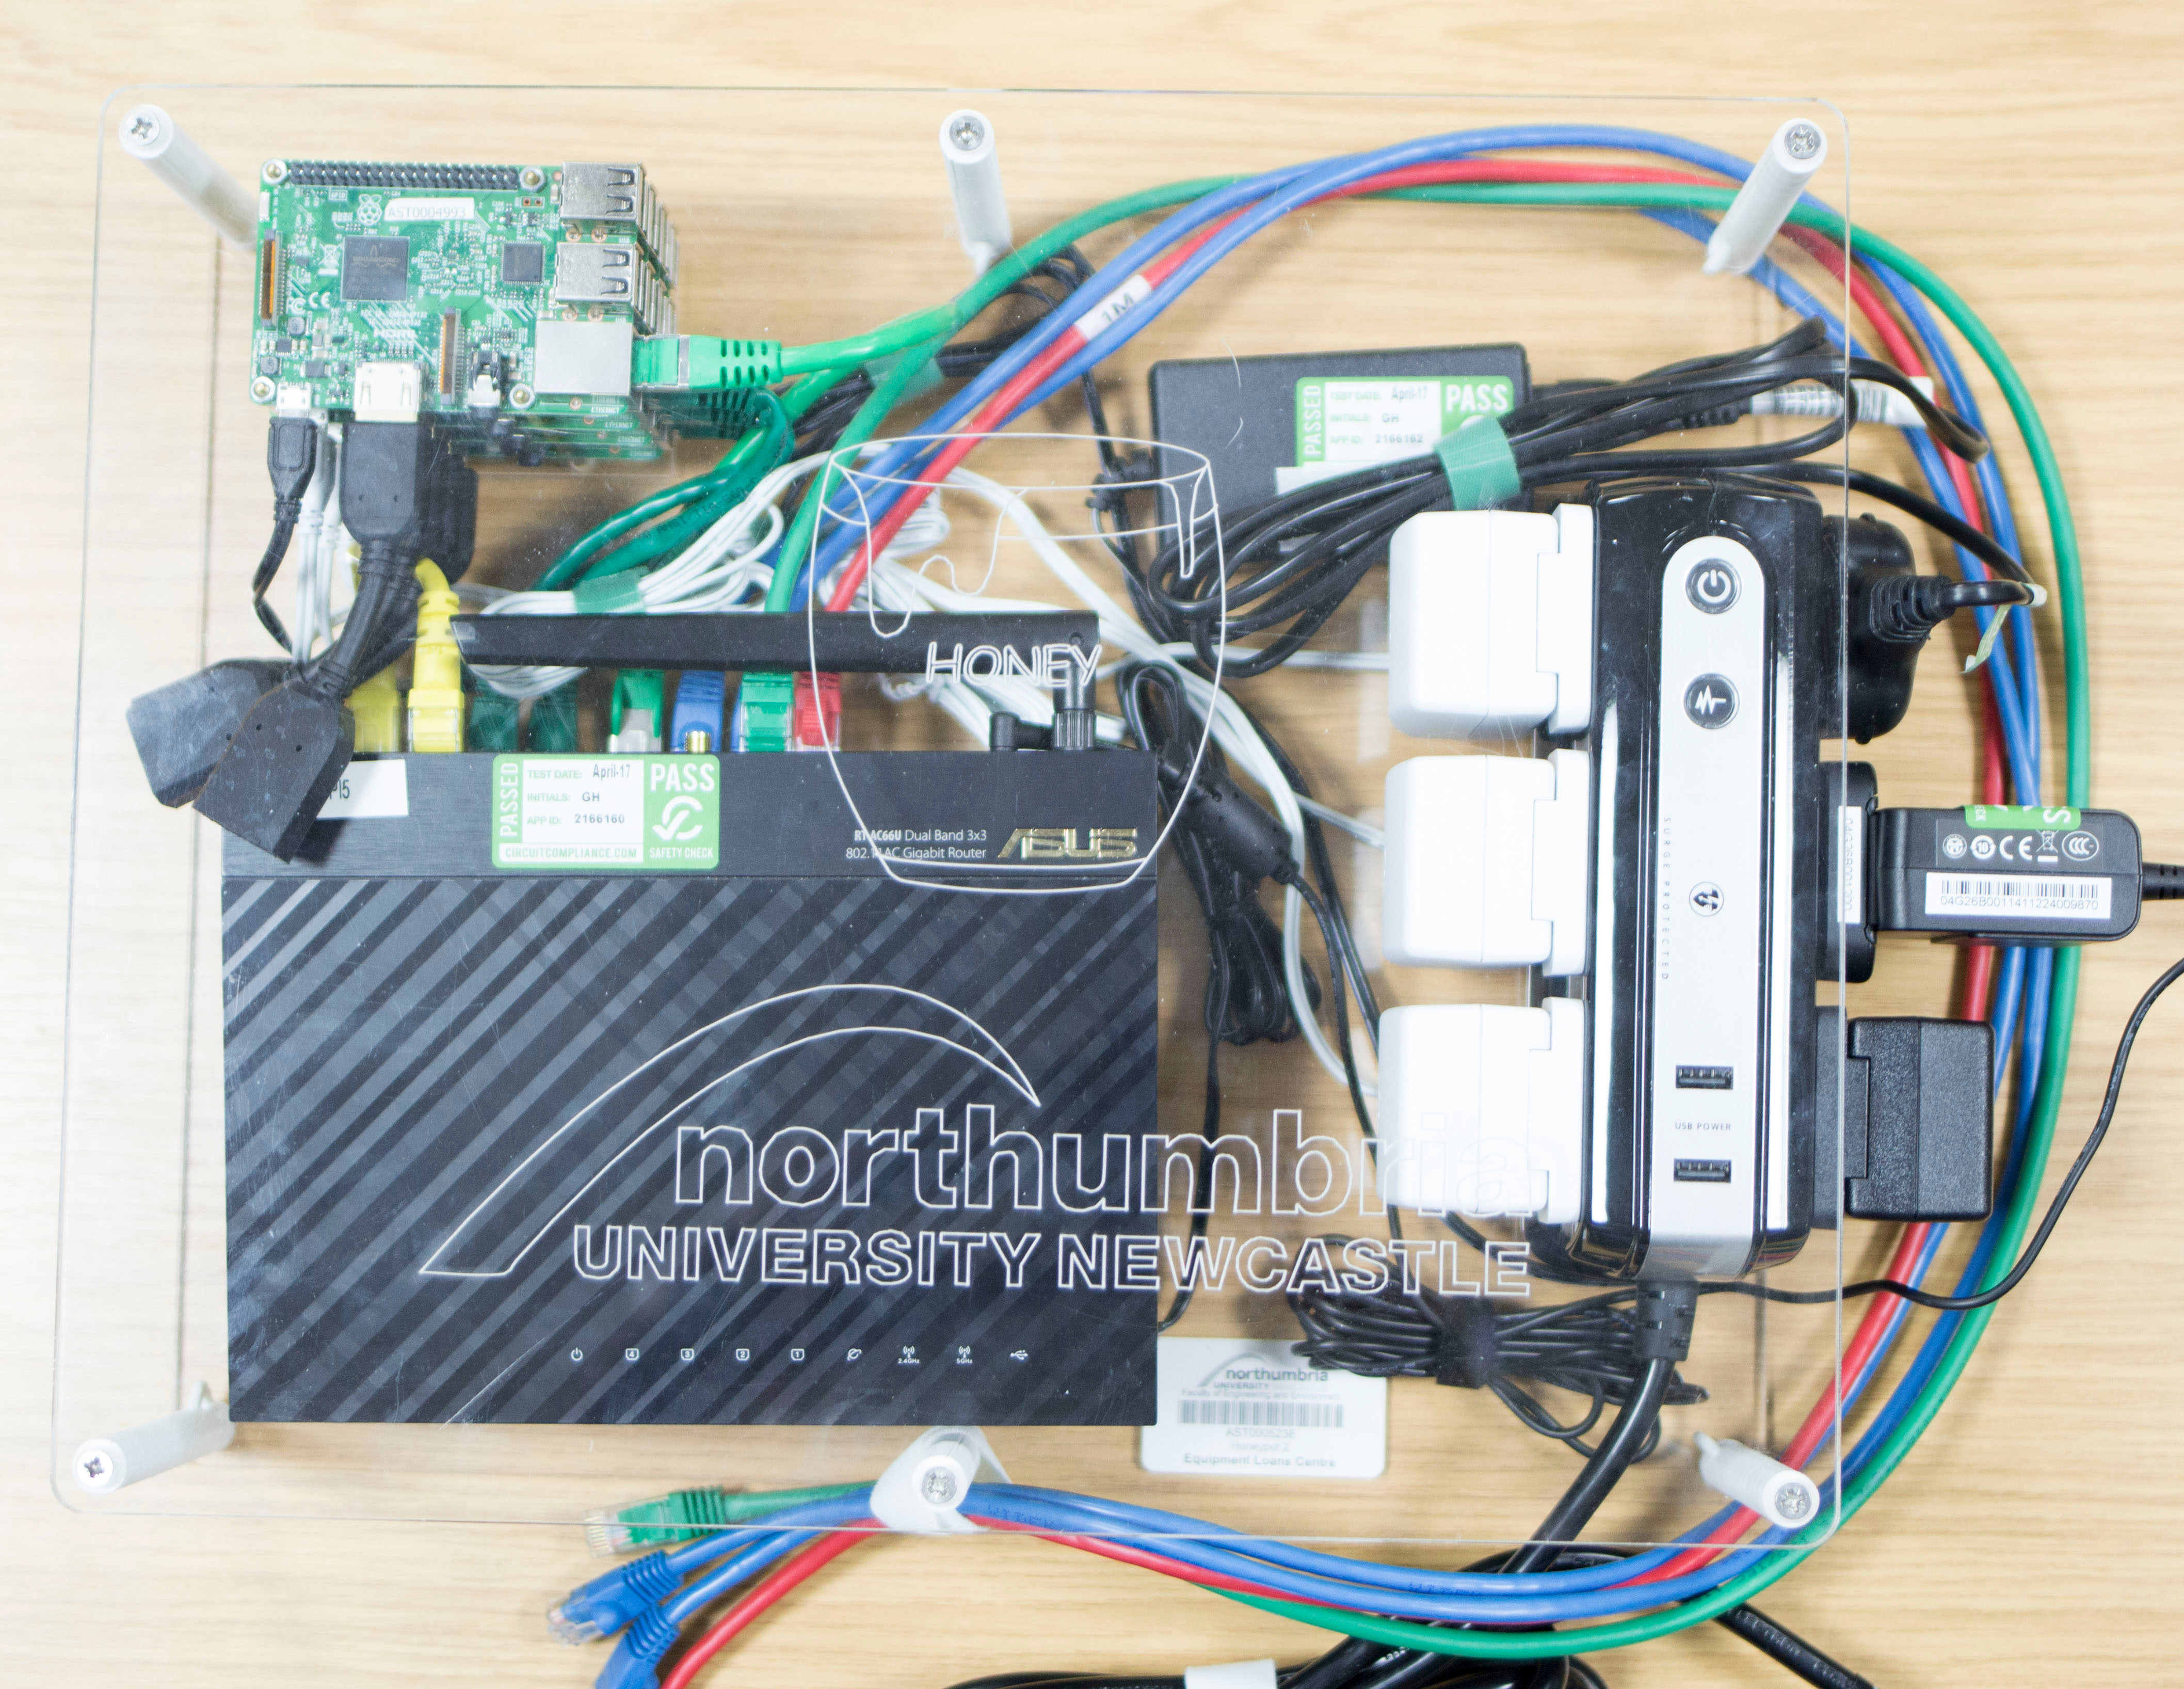
\includegraphics[width=\textwidth]{Images/HP2.eps}
    \caption{\texttt{HILV} top view}
    \label{fig:HP2}
  \end{minipage}
\end{figure}

%% \begin{figure}[htb]
%% \begin{center}
%% 	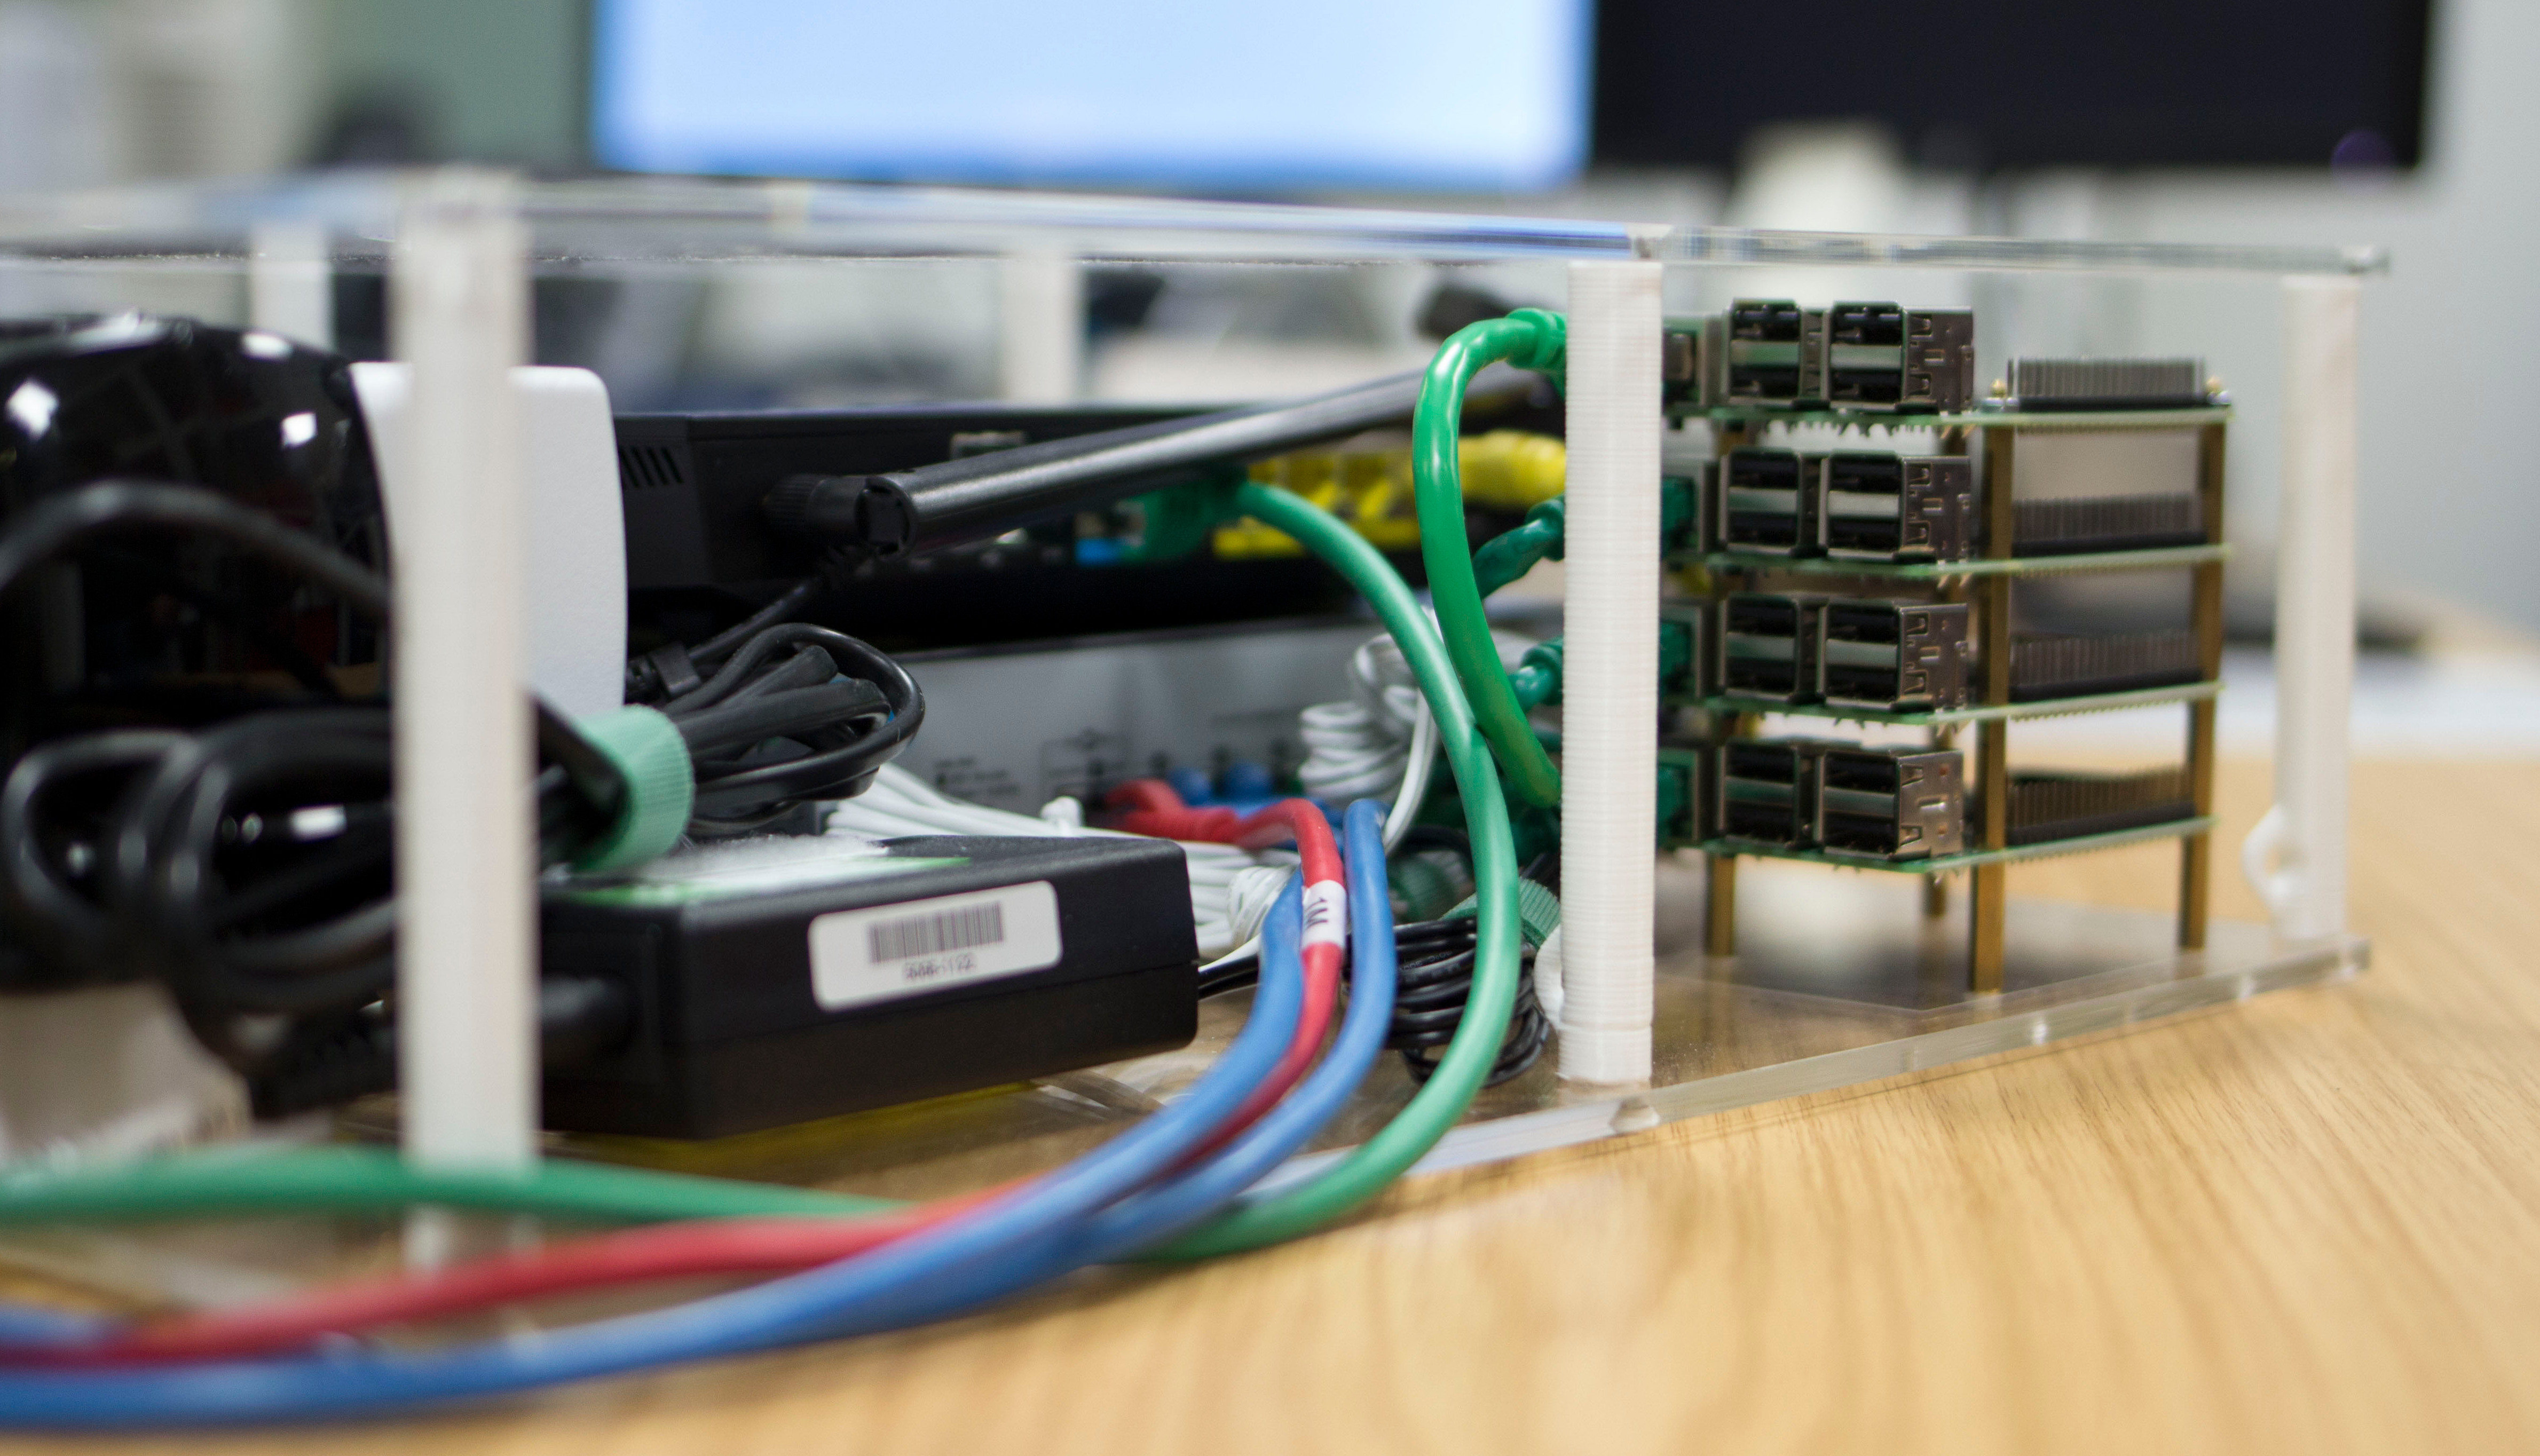
\includegraphics[scale=0.25]{Images/HP3.eps}
%% \caption{\texttt{HILV} Raspberry Pi boards (side view)}
%% \label{fig:HP3}
%% \end{center}
%% \end{figure}

Using Raspberry Pi boards as the main server technology within the honeypot has allowed reconfiguration and rebuilding of the architecture to be simplified. The operating system (and configured services) are stored on removable media (micro SD cards) which simplifies server recovery and the maintaining of multiple configurations. Images of the honeypot's base configuration can easily be restored. Multiple configuration can be kept on different image sets and students can keep individual projects as a set of micro SD cards that they retain for the duration of a project.

\subsubsection{Address range support}
The \texttt{HILV} honeypot environment must reside on a different subnet address for the double \texttt{NAT}'d configuration to function correctly. This is achieved by assigning a private, class A \texttt{IP} range providing more than 16 million addresses.

\subsubsection{Router configuration}
The \texttt{HILV} honeypot's \texttt{ADSL} router is configured to provide only routing services by disabling all other services for example \texttt{NAS} and \texttt{DHCP} facilities. This configuration allows all infrastructure protocols to be managed from within the honeypot using small scale servers (Raspberry Pi boards \cite{RASP:17}). Configuring the services on separate servers allows analysis of inter-service activity during normal network activity and during an attack.

The router used in the \texttt{HILV} honeypot is an ASUS RT AC66U~\cite{ASUS:17}. The router is configured to use laboratory based \texttt{DHCP} server to acquire an  address. The \texttt{IP} address is allocated from a reservation which allows a consistent mapping of the forwarded \texttt{IP} address from the internet based router to the research honeypot router. Defining the mapping in this way allows external host names (\texttt{URL}s) to be mapped to the honeypot for internet based attack analysis. Forwarding of the traffic from the research router into the honeypot can be enabled and disabled when required. 

For direct access to the honeypot from the laboratory \texttt{IP} forwarding is configured such that it will ``point" to a target machine within the honeypot as shown in Figure~\ref{fig:Forward}. In small scale routers this operation is normally referred to as a \texttt{DMZ} (demilitarised zone) redirection~\cite{DK:08,MB:01}. 

\begin{figure}[h]
\begin{center}
	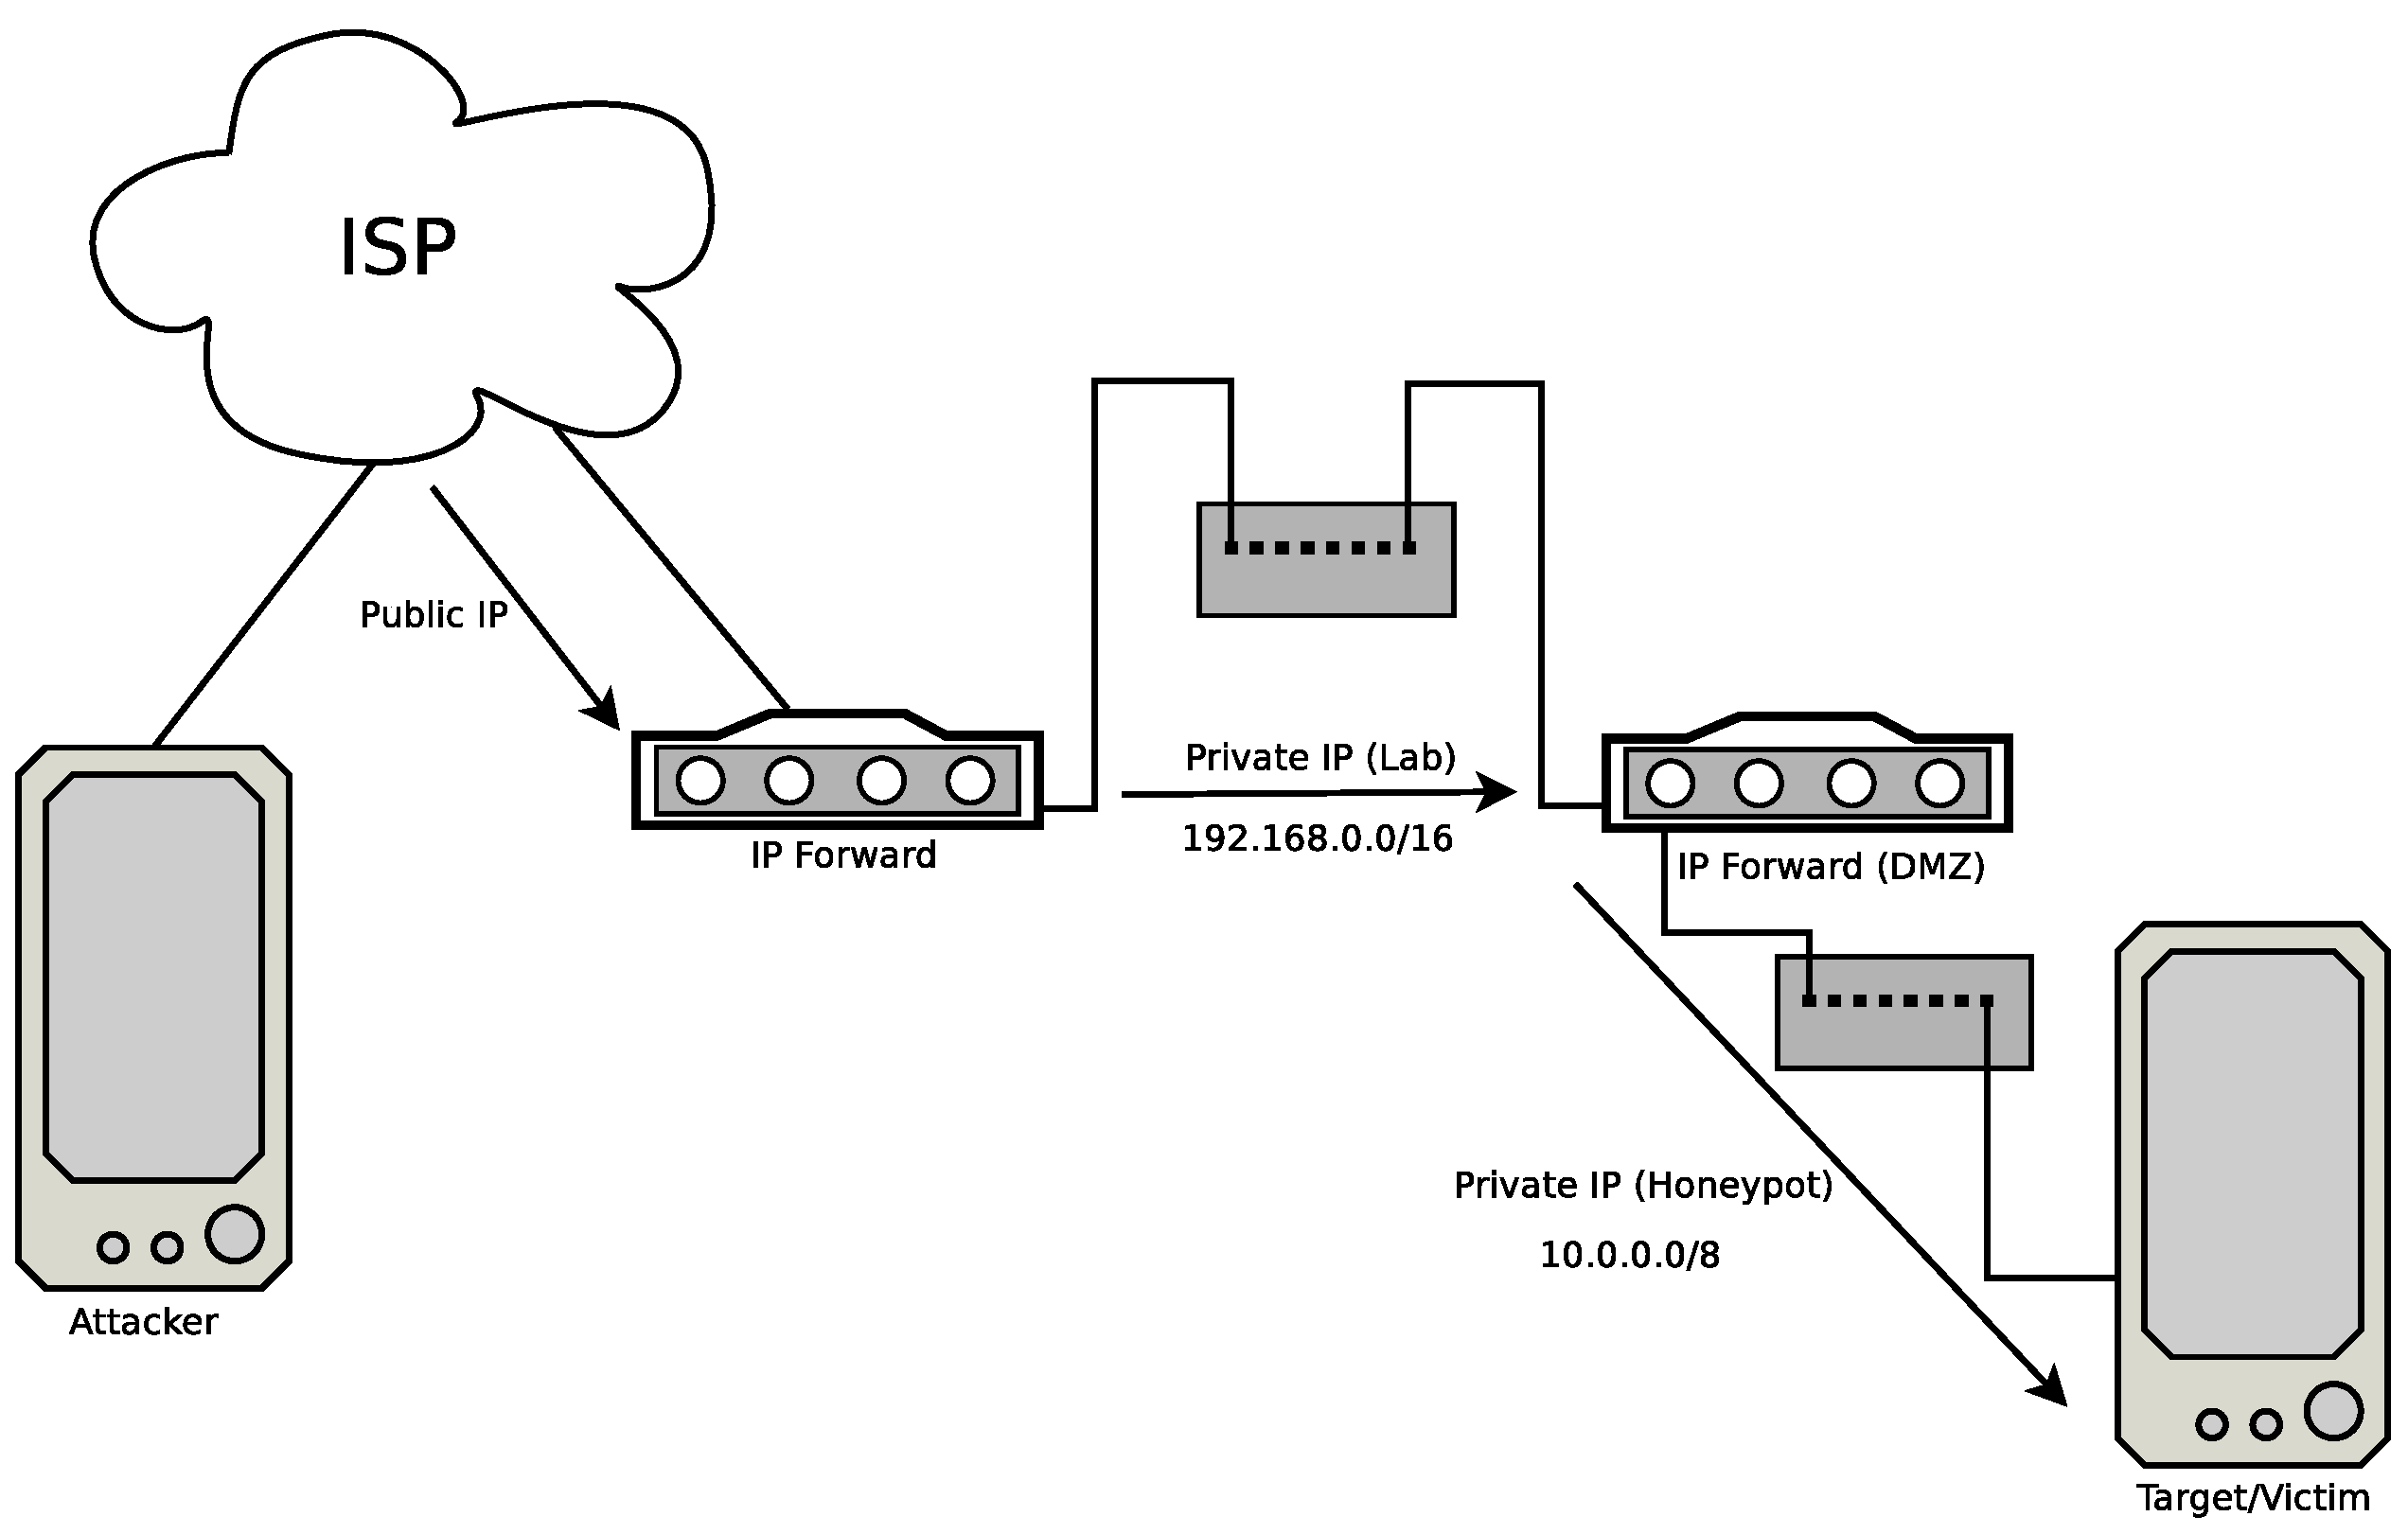
\includegraphics[scale=0.25]{Images/Forward.eps}
\caption{Address/Port forwarding}
\label{fig:Forward}
\end{center}
\end{figure}

\subsubsection{Switch configuration}
The main component of the \texttt{HILV} honeypot is a commercially available 8 port managed switch. The switch must support layer 2 management~\cite{ST:98} to provide two specific technologies: port mirroring and port throttling. Suitable switches include HP 2530-08~\cite{HP:17} or TP-LINK TL-SG2008~\cite{TP:17}. Port mirroring and port throttling combined provided a reliable packet capture architecture.
\newline\newline
\noindent\textit{Port mirroring}
\newline\newline
Switches by design provide a layer of security through virtual circuits. A virtual circuit is an internal route whereby traffic is filtered by the \texttt{Ethernet\_II} frame header. Switches maintain an in-memory table of ports and \texttt{MAC} addresses to route each packet to a specific port. The result of this routing is that packets are transferred port to port and not broadcast, which limits packet capture. When using a Honeypot packet capture is a vital part of the architecture for analysis of any network based attack vector. Using a managed switch (as discussed above) it is possible to configure the ports on the switch to be mirrored to a specific port as shown in Figures~\ref{fig:HPOverview} and \ref{fig:throttling}. This allows all the network activity to be captured and analysed~(\emph{Requirement 8}). 
\newline\newline
\noindent \textit{Bandwidth throttling}
\newline\newline
A further issue with capturing the packets within the honeypot that must be addressed is packet loss on the port where the mirrored traffic is forwarded. Switches by design endeavour to provided the maximum transfer speed possible between ports. This is achieved through the switch's backplane. The mirroring of packets has a lower priority than that of throughput and therefore packet loss on a mirrored port is inevitable on a heavily loaded switch. To prevent this occurring the switch must be configured to throttle the throughput on the mirrored ports so as not to overwhelm the backplane. Figure~\ref{fig:throttling} shows the basic configuration of a throttled environment. The port which has the packets forwarded to it must be configured to run at a speed that exceeds the total bandwidth of the mirrored ports. The effect of this is that as packets are transferred between ports they are reliably replicated via the backplane to the monitor port. This configuration satisfies \emph{requirement 8}.

\begin{figure}[h]
\begin{center}
	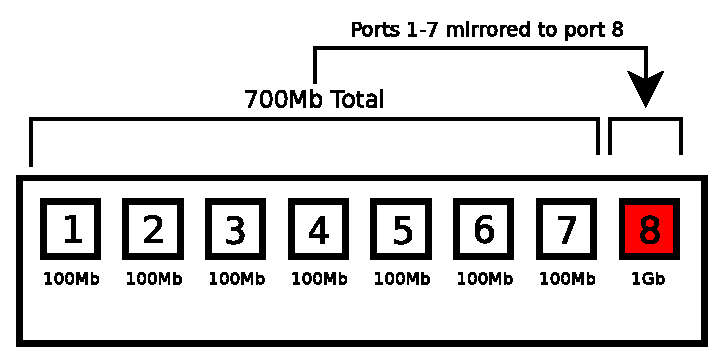
\includegraphics[scale=0.4]{Images/Throttle.eps}
\caption{Port throttling}
\label{fig:throttling}
\end{center}
\end{figure}

Switches can implement mirroring in two ways. Firstly as a monitor-only port where the transmission functionality of port is removed therefore no data can be transmitted to the infrastructure (as in the case of an HP 1810-G). This type of configuration therefore prevents a monitoring piece of equipment from adding traffic to the network. Alternatively some manufacturers setup the mirrored too port so it provided full functionality as well as the mirrored capability (as in the case of a TP-SG2008). This allows the attached monitor to also be used as a device within the honeypot. If the monitor port provides full functionality the addition of a LAN tap~\cite{RB:13} can remove the transmission facilities of the port creating the required monitor only functionality as shown in Figure~\ref{fig:HPOverview}.

\subsubsection{Internet support}
Access to the internet from the honeypot is possible through the double \texttt{NAT}'d configuration. The configuration provides isolation from the laboratory and the internet. Direct access to a target resource from the internet into either the laboratory based honeypot or into a small scale research honeypot is achieved through packet forwarding as shown in Figure~\ref{fig:Forward}. For this technique to function correctly the laboratory network and honeypot networks must be different subnets.

The internet facility also supports \texttt{IP} address forwarding to allow internet based access into the research honeypots. From the internet packets are forwarded to the address of a honeypot router which is in turn forwards traffic to a target machine inside the research honeypot as shown in Figure~\ref{fig:Forward}. 

This configuration allows specific configurations to be exposed to capture internet based attacks and to support remote access to the honeypot for remote configuration and monitoring.

\subsection{\texttt{LIHV} Honeypot}

The \texttt{LIHV} is not intended for use in a reconfigurable environment and does not require any monitoring or control of the network. No port monitoring or throttling is required and all activity monitoring is achieved using log file monitoring. The log files are made available on request for analysis of service based access activity.
 
The \texttt{LIHV} honeypot is located in a separate cabinet, shown in Figure~\ref{fig:Overview2}. The cabinet is secured to prevent students having direct access to the hardware. It supports the general service-base honeypot to provide students with a platform to carry out simple authentication attacks using tools such as \texttt{Hydra} from within the \texttt{Kali Linux}~\cite{OS:17} toolset. This honeypot also provides a target for the development of bespoke authentication attack tools in the final year undergraduate cyber-security modules.

\begin{figure}[h]
\begin{center}
	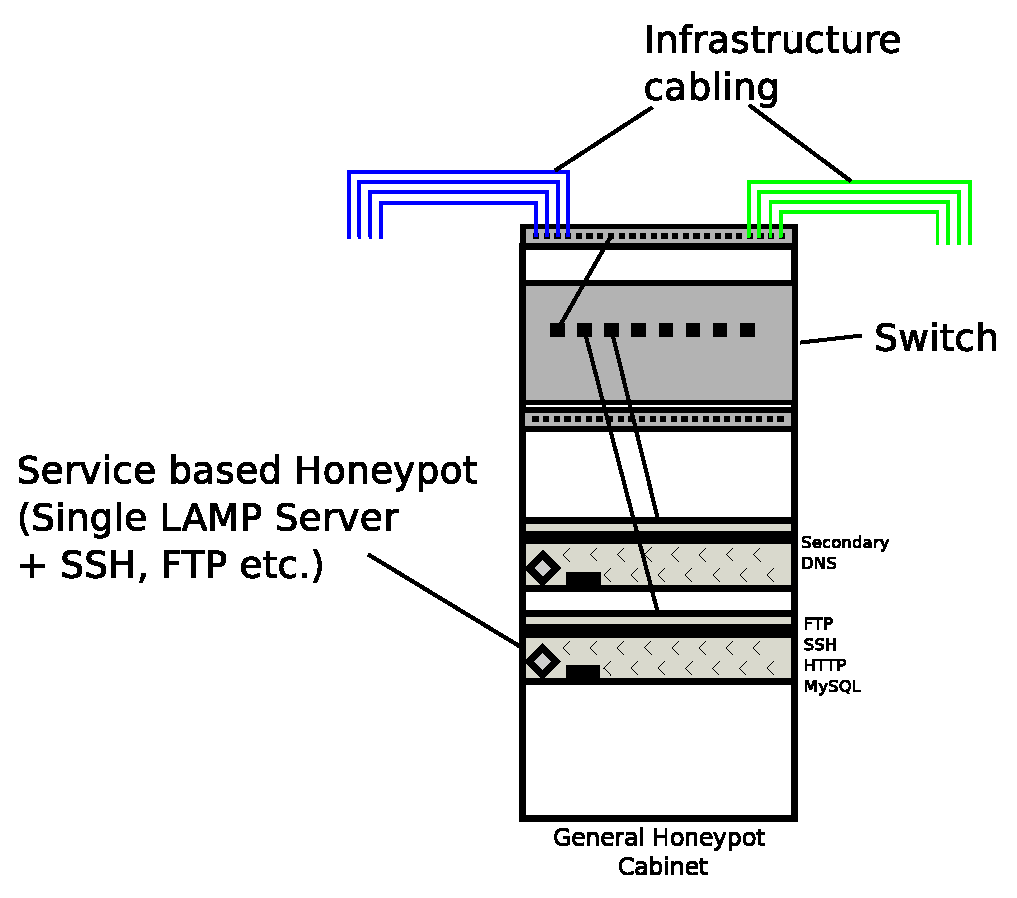
\includegraphics[scale=0.4]{Images/Infrastructure2.eps}
\caption{Laboratory general purpose honeypot overview}
\label{fig:Overview2}
\end{center}
\end{figure}

\subsubsection{Laboratory-based honeypot}
The \texttt{LIHV} honeypot is a single 1U \texttt{LAMP} server (Figure~\ref{fig:Overview2}). This server is accessed directly in the laboratory or via the internet as a bastion server~\cite{MB:05} through \texttt{IP} forwarding from the internet router. The server is used primarily for authentication attack projects based on dictionary attacks and scanning based reconnaissance, for instance, with Nmap~\cite{GFL:09} or service analysis tools such as WPScan~\cite{WT:17}. These types of attacks have a low impact on the network as a whole and are therefore safe to run in the general purpose laboratory. This machine is available internally and externally from the laboratory to allow directed learning tasks and also to support collaborative ventures.

\section{Operational results}\label{Results}
The base infrastructure has been in place, and actively used, for 10 years. The laboratory-based honeypot has been in place for 9 years. The honeypot was introduced to support the undergraduate networking program when the cyber-security module was introduced. This module was added to the BSc (Hons) Ethical Hacking degree 9 years ago in 2008.

The (\texttt{LIHV}) honeypot has been successfully used in the teaching of basic attack vectors such as port analysis, banner grabbing and service interaction (\texttt{FTP} and \texttt{HTTP}) for modules and projects. 

The (\texttt{HILV}) honeypots were designed and built 6 years ago and have been used since 2012 (5 years) on both the undergraduate networking and ethical hacking courses. The have been deployed in activities such as service redirection attacks, amplification attacks and man-in-the-middle scenarios.

The (\texttt{HILV}) research honeypots using Raspberry Pi boards has allowed diverse subjects to be taught more easily due to their use of removable media to store the operating system. The setup time for laboratories and teaching sessions has been dramatically reduced compared to using small clusters of PC's with removable drives. 

There have been several hardware changes to the (\texttt{HILV}) research honeypots over this time but the basic architecture has remained unchanged. The latest change was a Raspberry Pi 2 to Raspberry Pi 3 upgrade. The cost of layer 2 switches and their availability has also improved and are now more affordable. As new honeypots are fabricated TP-LINK switches are being used in reference to the more expensive HP switches. The TP-LINK switches do not provide a fully implemented monitor port, this necessitates the need for the inclusion of a network tap as shown in Figure~\ref{fig:HPOverview}.

\subsection{Current resource support}\label{ResourceSupport}
The current implementation of the laboratory supports $>200$ students. This includes undergraduate programs covering networking ($\sim40$), networking and cyber-security ($\sim150$) and postgraduate programmes covering networking ($\sim20$). Each of these programmes are modularised (broken down into modules).  A typical undergraduate programme runs around $10$ modules concurrently e.g. networking technology (years 1, 2, 3 \& 4 with MComp), security case projects (Year 2), Sockets programming (year 3). Each module requires $\sim3$ hours contact per week and $\sim3$ hours of directed learning, which may require laboratory time. In addition the laboratory supports many undergraduate and post graduate cyber-security projects ($\sim80$) including cyber attack analysis and general cyber-security research such as biometric-based multifactor authentication and \texttt{IoT} (Internet of Things) security projects.

\subsection{Supported Modules}\label{Modules}
All network engineering modules across both undergraduate and postgraduate programmes involving routing, switching, \texttt{VLAN} deployment, \texttt{MPLS} networking and \texttt{IP} telephony are all successfully taught using the general networking laboratory infrastructure. 

Network service deployment using server operating systems (Windows and Linux) for both undergraduate and postgraduate programmes are taught successfully in the environment using virtual machine technologies. The network service deployments include load-balanced \texttt{HTTP}, network file system deployments (\texttt{NFS} and \texttt{SMB}), replication based \texttt{MySQL} services and large scale \texttt{DNS} deployments.  

The \texttt{HILV} honeypot environment has allowed aspects of network based infrastructure, specifically broadcast based network services, to be taught as a practical implementation rather than simulations and has allowed students to develop complete infrastructures integrated to the internet.

Cyber-security modules are predominantly taught using the research-honeypot platform specifically when looking at attack vectors that require packet spoofing or resource exhaustion through high volume traffic generation.

The \texttt{HILV} honeypots have also allowed analysis of live attacks from the internet without impacting on the local laboratory network. Activities such as port scanning are passed through directly to the research honeypot without exposing the laboratory infrastructure. Implementing multiple research honeypots has allowed profiles of subnet scanning and attacks to be analysed by students and have provided them with a rich environment for experimentation and analysis.    

\subsection{Supported projects}\label{Projects}
The most prolific area of usage of the research honeypot platforms is in the area of cyber-security research projects some of which are listed below: 
\begin{itemize}
\item \noindent \emph{Multi-Tiered defence analysis of a simulated cyber attack.} - This project involved configuring the research honeypots to support a \texttt{IPFire} (software based firewall technology) and investigating potential tunnelling techniques that could compromise a military grade network deployment.
\item \noindent \emph{Development of a small \texttt{IDS}.} This project involved developing a libpcap based application to run on one of the honeypot Raspberry Pi's (v3)~\cite{RASP:17} that could monitor network traffic to identify a \texttt{SYN} flood attack using a basic window based statistical analysis.
\item \noindent \emph{Attack on a secure \texttt{IoT} protocol} This project involved developing a network of \texttt{IoT} devices for environment analysis (temperature and humidity) and identify the encrypted traffic (\texttt{MQTT}) which was then attacked using a block decryption technique.
\item \noindent \emph{Development of an \texttt{IDS} for a full subnet \texttt{MitM} attack} This project involved developing a stateful based \texttt{IDS} using libpcap to identify spoofed \texttt{ARP} packets.
\item \noindent \emph{Development of a \texttt{DOS} tool that attempts to prevent detection from an \texttt{IDS}} This project involved developing a \texttt{RAW} sockets based application that crafted packets to replicate valid traffic within the subnet environment.
\item \noindent \emph{Analysis of a \texttt{DNS} amplification} This project involved configuring a vulnerable \texttt{DNS} environment and executing an attack and analysing the bandwidth effect of the network.
\end{itemize}

\section{Conclusion and Future work}\label{Future}
The development of the \texttt{HILV} honeypot environment has proved successful for both teaching and research. The cost of the deployment has been minimised to such an extent that rather than the laboratory supporting a single honeypot platform, which has to be reconfigured between sessions, the laboratory can now support multiple honeypot deployments that are highly configurable and portable. 

As the \texttt{HILV} honeypots are small scale and low cost the equipment is permanently configured for teaching purposes. Each \texttt{HILV} honeypot is capable of supporting four students at a time to work on research based modules and allows practical cyber-security modules to be delivered more effectively.

Student numbers have risen sharply for cyber-security-specific courses and the use of the honeypots has allowed additional levels of cyber-security to be incorporated into existing network courses. This has had a strategic impact on the University since the B.C.S. (British Computing Society) added cyber-security as a required part of its accreditation process. 

The aim going forward is to increase the number of \texttt{HILV} honeypots to accommodate the increasing number of students. Due to the architecture being low cost this is an achievable goal. It is also envisaged that using this technology the department will be able to expand its cyber-security based research by recruiting PhD students in the subject area to work on diverse projects that will require significantly different honeypot configurations by introducing a \texttt{HIHV} honeypot deployment. This deployment will consist of several large scale servers along with commercial grade switches and routers and large scale data capture facilities.  

%% \paragraph{Paragraph headings} Use paragraph headings as needed.
%% \begin{equation}
%% a^2+b^2=c^2
%% \end{equation}

%% % For one-column wide figures use
%% \begin{figure}
%% % Use the relevant command to insert your figure file.
%% % For example, with the graphicx package use
%%   \includegraphics{example.eps}
%% % figure caption is below the figure
%% \caption{Please write your figure caption here}
%% \label{fig:1}       % Give a unique label
%% \end{figure}
%% %
%% % For two-column wide figures use
%% \begin{figure*}
%% % Use the relevant command to insert your figure file.
%% % For example, with the graphicx package use
%%   \includegraphics[width=0.75\textwidth]{example.eps}
%% % figure caption is below the figure
%% \caption{Please write your figure caption here}
%% \label{fig:2}       % Give a unique label
%% \end{figure*}
%% %
%% % For tables use
%% \begin{table}
%% % table caption is above the table
%% \caption{Please write your table caption here}
%% \label{tab:1}       % Give a unique label
%% % For LaTeX tables use
%% \begin{tabular}{lll}
%% \hline\noalign{\smallskip}
%% first & second & third  \\
%% \noalign{\smallskip}\hline\noalign{\smallskip}
%% number & number & number \\
%% number & number & number \\
%% \noalign{\smallskip}\hline
%% \end{tabular}
%% \end{table}


%\begin{acknowledgements}
%If you'd like to thank anyone, place your comments here
%and remove the percent signs.
%\end{acknowledgements}

% BibTeX users please use one of
%\bibliographystyle{spbasic}      % basic style, author-year citations
\bibliographystyle{spmpsci}      % mathematics and physical sciences
%\bibliographystyle{spphys}       % APS-like style for physics
\bibliography{honeypot}   % name your BibTeX data base

% Non-BibTeX users please use
%\begin{thebibliography}{}
%
% and use \bibitem to create references. Consult the Instructions
% for authors for reference list style.
%
%\bibitem{RefJ}
% Format for Journal Reference
%Author, Article title, Journal, Volume, page numbers (year)
% Format for books
%\bibitem{RefB}
%Author, Book title, page numbers. Publisher, place (year)
% etc
%\end{thebibliography}

\end{document}
% end of file template.tex

